%
% File acl2019.tex
%
%% Based on the style files for ACL 2018, NAACL 2018/19, which were
%% Based on the style files for ACL-2015, with some improvements
%%  taken from the NAACL-2016 style
%% Based on the style files for ACL-2014, which were, in turn,
%% based on ACL-2013, ACL-2012, ACL-2011, ACL-2010, ACL-IJCNLP-2009,
%% EACL-2009, IJCNLP-2008...
%% Based on the style files for EACL 2006 by 
%%e.agirre@ehu.es or Sergi.Balari@uab.es
%% and that of ACL 08 by Joakim Nivre and Noah Smith

\documentclass[11pt,a4paper]{article}
\usepackage[hyperref]{acl2019}
\usepackage{times}
\usepackage{latexsym}

\usepackage{url}
\usepackage{listings}
\usepackage{color}
\usepackage{graphicx}
\definecolor{dkgreen}{rgb}{0,0.6,0}
\definecolor{gray}{rgb}{0.5,0.5,0.5}
\definecolor{mauve}{rgb}{0.58,0,0.82}

\lstset{frame=tb,
  language=Python,
  aboveskip=3mm,
  belowskip=3mm,
  showstringspaces=false,
  columns=flexible,
  basicstyle={\small\ttfamily},
  numbers=none,
  numberstyle=\tiny\color{gray},
  keywordstyle=\color{blue},
  commentstyle=\color{dkgreen},
  stringstyle=\color{mauve},
  breaklines=true,
  breakatwhitespace=true,
  tabsize=3
}
\aclfinalcopy % Uncomment this line for the final submission
%\def\aclpaperid{***} %  Enter the acl Paper ID here

%\setlength\titlebox{5cm}
% You can expand the titlebox if you need extra space
% to show all the authors. Please do not make the titlebox
% smaller than 5cm (the original size); we will check this
% in the camera-ready version and ask you to change it back.

\newcommand\BibTeX{B\textsc{ib}\TeX}

\title{Text Classification for Task-based Source Code Related Questions}

\author{
  Siddhartha Punj \\ \And
  Jailan Sabet \\ \And
  Jinxiao(Jason) Song\\ \AND
  David Tomassi\\ \And
  Sairamvinay Vijayaraghavan}

\date{}
\begin{document}
\maketitle
\section{Introduction}
Classification of text is an important field of research and a core
task in Natural Language Processing (NLP). It spans many different
domains from determining “fake” news, finding spam emails, and
language detection. A common problem in software development is
finding the appropriate code snippet for a task. There are communities
for software development that allow people to ask questions and
provide answers such as Stack Overflow. The issue that arises is that
many people will provide completely different answers for a particular
question in which many cases the answers are wrong. We pose the task
of determining if a pair of a question/problem and  a corresponding
code snippet is appropriate or not as a binary classification problem.

Our goal is to learn from these pairs the correct code snippets for
certain problems. An example of this is the code snippet,
\begin{lstlisting}
shutil.copy('file.txt', 'file2.txt')
\end{lstlisting} and the question, “Is this how this process where the task is to copy one file's contents to another in python?”. We will make use
of deep learning models to learn from a code corpus and corresponding
intent converted into ‘yes’ or ‘no’ labelled data. The creation of the
‘yes/no’ questions will be conducted by prepending “Is this how” and
similar wordings to make the intent into a question. We will have the
positive “yes” questions as the standard answer to the question. The
negative “no” questions will be created by sampling different code
snippets from other pairs and creating new pairs with these new code
snippets with the original question. So, we plan to ensure that an
equal number of positive and negative samples are used for training
our models for classification.

\section{Dataset}
For validating our hypothesis, we plan to choose working on a
Code/Natural Language Challenge (CoNaLa) dataset. This dataset
contains 598k samples in form of json lines formatted files automatically data mined from
StackOverflow which contains the question ID, intent of the code
snippet presented, code snippet, parent answer post ID, and an unique
ID for the post. In addition to the above set, there is another around 2K
samples of manual curated data which contains question ID, intent, rewritten
intent and also the code snippet. So, we plan to use the combination
of both these data sets. These datasets would provide all the snippets
in Python3 Programming Language.

\section{Baseline Model}
\begin{figure}
    \centering
    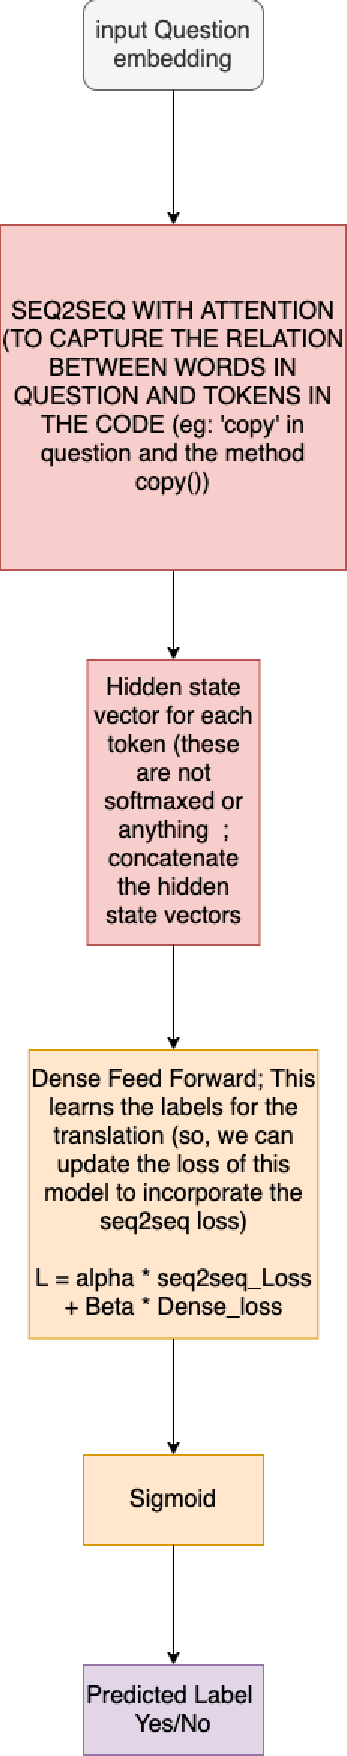
\includegraphics[height=10cm,width=4cm]{ModelPipeline.pdf}
    \caption{The overall pipeline of our project}
    \label{fig:my_label}
\end{figure}



\subsection{Model Description}
This project is a binary classification task which will be under supervised learning by having a label for each pair of question and code snippet. Since we use the CoNALA dataset, the CoNaLa will provide the intent
which is the input question sequence and the output code snippet as
the context information. Then, we will process the input question by
prepending some interrogative words (such as the common phrase “is
this how this process...”) in front of the input sequence which will
convert it into the question format. For the code, we won’t be doing a
lot of work but we will break it up into tokens which are
understandable by the machine (code can be broken up into tokens for
learning the structure of the code done for a task).

We plan to alter these datasets in order to suit to our task by
performing some additions to the intent by rephrasing it as a question
while we utilize the appropriate snippet as a context to formulate the
problem to be solved and then add labels as “yes” or “no” for training
our models.

We plan to also use further analysis for developing the context
related vocabulary by using a code related corpus which provides the
models to train by learning the vocabulary for analyzing the tokens
present in the Python3 Programming language. So for this task, we
intend to utilize a large Python3 vocabulary corpus which contains the
key tokens present in the programming language. For this, we intend to
use some different corpora: StaQC (stack overflow mined dataset QA
pairs but there is an extracted vocabulary file which we use); Code
Docstring corpus for extracting the vocabulary tokens useful for
learning the context related vocabulary. We are still in pursuit of
larger corpus for training our models but we will implement these
corpora as a base for building our contextual vocabulary for now.

Our problem setting is a sequence-to-sequence with attention model
where the input is a question sequence and the output is a code
sequence. We will map each question into a real vector domain, a
popular technique when working with natural language text called word
embedding. We plan to use some pre-trained word embeddings such as
GloVe or Word2Vec where words are encoded as real-valued vectors in a
high dimensional space, where the similarity/global contextual meaning
between words translates to closeness in the vector space. Then, we
can feed the hidden state vector from the seq2seq output to the
forward neural network model.  Forward neural network model will learn
the labels for the code snippet’s correctness since we will update the
loss of the model each time and incorporate the seq2seq loss together
in order to increase the learning performance. Then,using a dense
output layer with a single neuron, sigmoid activation function can
help to make 0 or 1 predictions for the two classes (correct and
incorrect) in the problem. 

\subsection{Model related training details}
In order to increase the performance of our training deep learning model, we can use the Adam optimizer. The Adam optimizer combines the effectiveness of AdaGrad, which improves performance on problems with sparse gradients, as well as RMSProp, which maintains parameter learning rates that are adapted based on how quickly the weights of the model are changing, which means it does well on noisy data (nonstandard words, missing punctuation, abbreviations, etc.). To summarize, it can modify the weight decay and learning rate of a model separately, which results in vastly improved general performance. Since we are working with a standard classification problem, we can use binary cross entropy as the loss function in order to determine how well the model classifies the data. In order to figure out the optimal architecture for the model, we will perform extensive hyper parameter search for finding the optimal hyper parameters. We will also use regularization within our classification sub model (the Dense Feed Forward Neural Network) for avoiding over-fitting.

Finally, in order to reduce time for training, we can potentially implement early stopping in the seq2seq model so that we break from the training loop early if the current validation loss happens to exceed the previous loss for determining whether a code snippet matches the rephrased task question or not in order to avoid overfitting.
\section{Evaluation}
In order to measure how effectively our model is able to classify CoNaLa rephrase question/snippet pairs accurately, we can use F1 scores, which utilizes both precision and recall. In addition, we will also use accuracy in order to calculate how accurately our model classifies a rephrased question with its correct code snippet. 

We have three proposed methods which we plan to use for evaluation. 
\subsection{Use the Original CoNaLa Dataset alone}
The first method involves using the original dataset, CoNaLa, by assigning only 80\% of the modified dataset to training our model and utilizing the remaining 20\% as a test set. This method would ensure that the training and test sets are consistent, but will contain the least amount of examples per set. This is a standard 80-20\% train-test split for evaluation on the original CoNaLa dataset.

\subsection{Adapt other corpora into CoNaLa from training}
For the second method, we can adapt other corpora, such as StaQC or Code Docstring, to construct a dataset separate from the training set; the modified dataset from CoNaLa, in this case, would all be used for training. This method would allow for larger datasets, but less consistency among the training and test sets. But we plan to use this for providing outer datasets helpful for evaluating generalization of the classification model.

\subsection{Raw Fresh dataset generated from Stack Overflow API}
Finally, for the last method, we intend to generate a completely new dataset by web scraping relevant websites, such as Stack Overflow, by crawling from the Stack Overflow API. This would involve adapting the raw collected data into a test set, leaving the various other corpora (such as CoNaLa, StaQC, and Code Docstring) available for training our model. This method would result in the large amount and variety of examples for the training and test set, but would be the least consistent and most time consuming.

\subsection{Additional test experiment as a real-life demo}
As a separate method of evaluating the model, we also plan to ask classmates to provide inputs (a snippet of code and a question about the code) for our classifier and report the overall accuracy of the total resulting outputs as well as the largest number of times our model consecutively determines the correct answer. This is more of a fun demonstration we plan to execute in class.

\begin{figure}
    \centering
    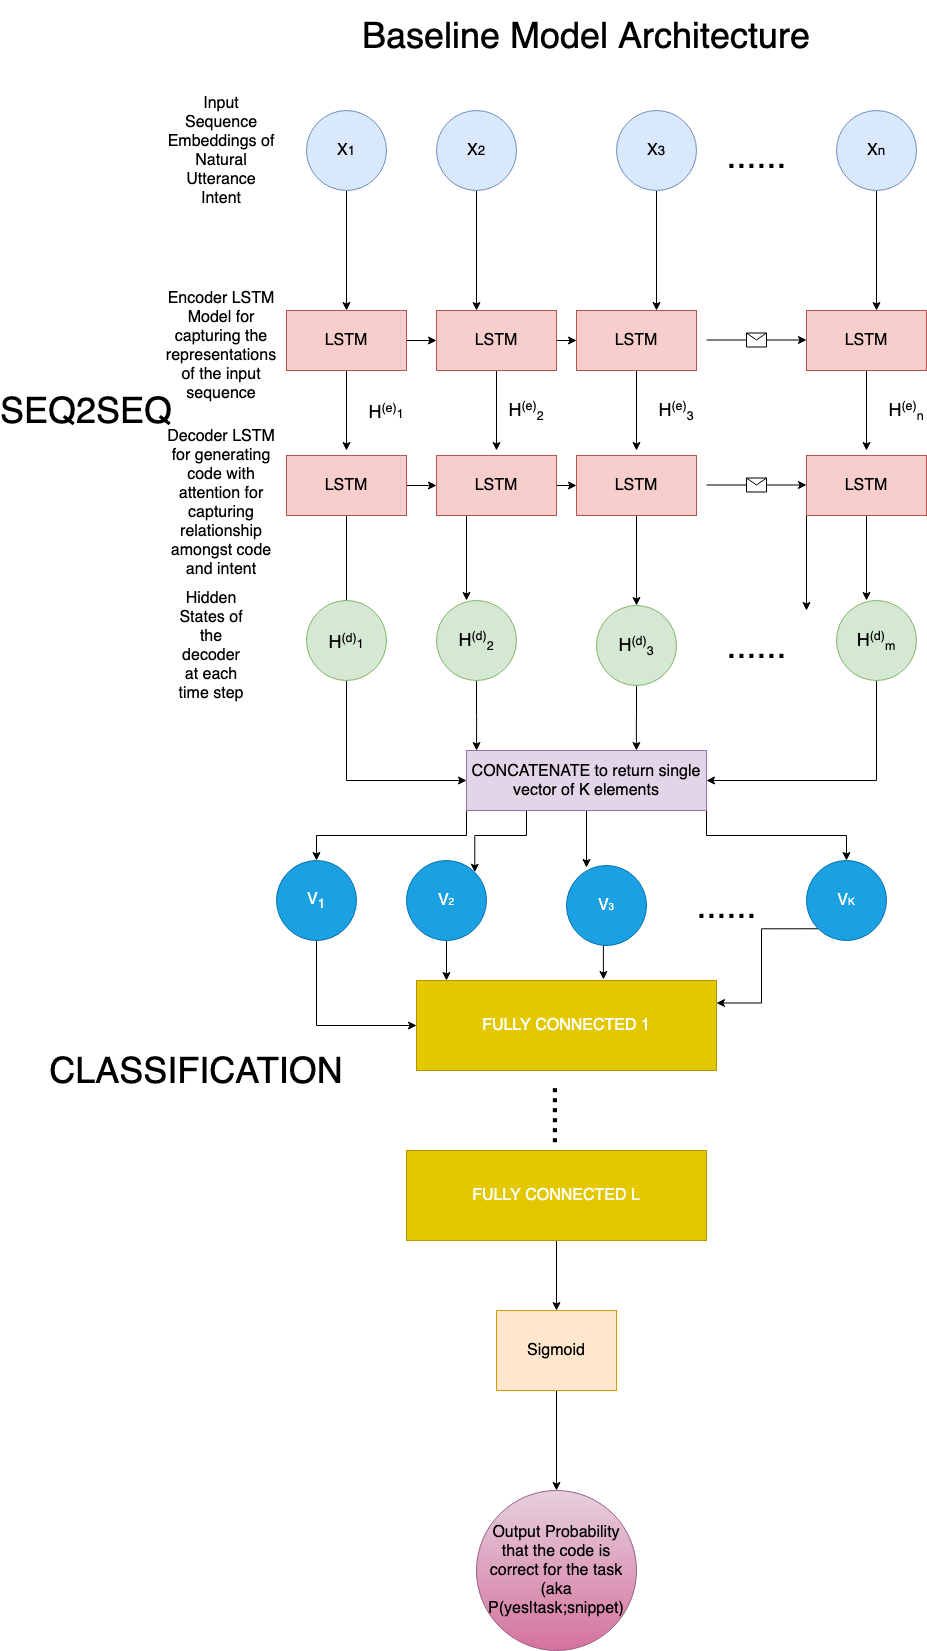
\includegraphics[height=20cm,width=10cm]{ModelArchitecture.png}
    \caption{The baseline model of our project}
    \label{fig:my_label}
\end{figure}

\section{References}
Yin, Pengcheng and Deng, Bowen and Chen, Edgar and Vasilescu, Bogdan and Neubig, Graham. Learning to Mine Aligned Code and Natural Language Pairs from Stack Overflow. 2018. https://doi.org/10.1145/3196398.3196408 \\ \\
Yao, Ziyu, et al. StaQC: A Systematically Mined Question-Code Dataset from Stack Overflow. Mar. 2018, arxiv.org/pdf/1803.09371.pdf. \\ \\
Barone, Antonio  Valerio Miceli. A Parallel Corpus of Python Functions and Documentation Strings for Automated Code Documentation and Code Generation. July 2017, arxiv.org/pdf/1707.02275.pdf. \\ \\
Yin, Pencheng. Neubig Graham. TRANX: A Transition-based Neural Abstract Syntax Parser for Semantic Parsing and Code Generation. October 2018. https://arxiv.org/abs/1810.02720 \\ \\


\end{document}
